\subsection{Implementering}

De centrale funktioner for kalenderen, for at operere på events ses nedenunder.

\begin{itemize}
    \item EventInsert
    \item GetEvents
    \item DeleteEvent
    \item GetUserEvents
\end{itemize}

De er centrale idet at de opfylder US kravene for kalender. Implementationen for de enkelte funktioner vil blive gennemgået kort og overordnet, hvor en dybere gennemgang af implementationen kan ses i bilagene under \cite{DesignOgImplementationCalendar}. 

\textbf{EventInsert}
\newline
\noindent 
For funktionen EventInsert, forsøges der først at indsætte eventet i databasen, og lykkes det returneres bruger til gruppekalenderen igen, hvor det kan ses at det nye event kommer på kalenderen over alle events. Lykkedes det ikke at indsætte eventet, returneres der NotFound for funktionen.

\textbf{GetEvents} 
\newline
\noindent 
Trinene for hvad der sker i funktionen for GetEvents kan ses på figur \ref{fig:GetEventsDiagram} og som det ses på figuren, er det første der tjekkes for om brugeren er en del af gruppen, da man skal have de events der gælder for gruppen. Det gøres ved at sammenligne parameteren for funktionen, som er gruppe id'et. Den anden parameter er en string som bruges til at bestemme event typen. 

\begin{figure}[H]
    \centering
    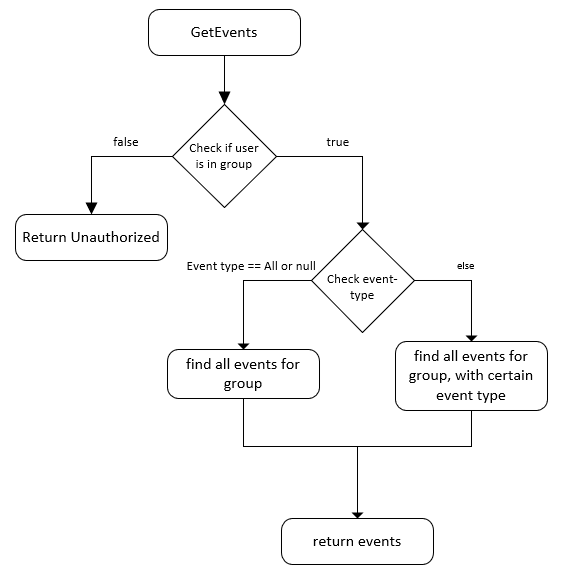
\includegraphics[width=0.8\linewidth]{10_Design_og_implementering/Calendar/Images/GetEvents.PNG}
    \caption{GetEvents diagram til Calendar}
    \label{fig:GetEventsDiagram}
\end{figure}{}

\textbf{DeleteEvent}
\newline
\noindent 
For funktionen DeleteEvent ledes der først efter eventet som ønskes slettet. Findes eventet i databasen, slettes det fra databasen, hvis ikke det findes, vil der ikke ske noget. Funktionen vil returnere true/false i Json format for at indikere status på funktionen, afhængig af om det lykkedes at slette eventet eller ej. 

\textbf{GetUserEvents}
\newline
\noindent
I funktionen GetUserEvents findes først den bruger som er logget ind, og herefter laves en Sql join sætning. %\ref{list:calendar_getUserEvents}


%\lstinputlisting[label={list:calendar_getUserEvents},caption=Implementering af GetUserEvents.]{10_Design_og_implementering/Calendar/Code/GetUserEvents.cs}

Først og fremmest joines der på Events og GroupsUsers tabellen på matchende gruppeId, herefter finder vi de events deriblandt hvilken tilsvarende GroupsUsers tabel samtidigt har et UserId som er tilsvarende den user som nuværende er logget ind. Til sidst læses alle attributer fra disse events over i en liste, som vi returnerer til javascriptet i JSON format.
